%%%%%%%%%%%%%%%%%%%%%%%%%%%%%%%%%%%%%%%%%
% Beamer Presentation
% LaTeX Template
% Version 1.0 (10/11/12)
%
% This template has been downloaded from:
% http://www.LaTeXTemplates.com
%
% License:
% CC BY-NC-SA 3.0 (http://creativecommons.org/licenses/by-nc-sa/3.0/)
%
%%%%%%%%%%%%%%%%%%%%%%%%%%%%%%%%%%%%%%%%%

%----------------------------------------------------
%	PACKAGES AND THEMES
%----------------------------------------------------

\documentclass{beamer}

\usepackage{graphicx}
\usepackage{hyperref}

\newcommand{\ket}[1]{\left|{#1}\right\rangle}

\setbeamertemplate{navigation symbols}{}
\usetheme{Madrid}
\definecolor{QiskitPurple}{rgb}{0.412, 0.161, 0.769} 
\usecolortheme[named=QiskitPurple]{structure}

%-----------------------------------------
%	TITLE PAGE
%-----------------------------------------

\title[Quantum Discrete Logarithm Algorithm]{A New Quantum Solution to the Discrete Logarithm Problem}

\author[The Josephson Junctions]{Matthew Gregoire \inst{1} \and Richard Howe \inst{2} \and Guan-Wen Chou \inst{2} \and Anton Nikulsin \inst{2}}
\institute[Summer Jam]{
\inst{1}UNC Chapel Hill \and
\inst{2}North Carolina State University
}
\date{\today}

\begin{document}

\begin{frame}
\titlepage
\end{frame}

%------------------------------------------------
%	PRESENTATION SLIDES
%------------------------------------------------

\begin{frame}{The Discrete Logarithm Problem}

Take a modulus $N$, an integer $a$, and a power $b$ of a, such that $b = a^m \mod N$.

\begin{block}{The Discrete Logarithm Problem}
Given the values $a$ and $b$ mod $N$ as above, find the value of $m$.\footnotemark
\end{block}

\begin{itemize}
    \item It's easy to compute $b$ when given $a$ and $m$.
    \item It's hard to find $m$ when given $a$ and $b$.
    \item This fact is the basis of many modern cryptographic protocols.
\end{itemize}

\footnotetext[1]{This can actually be generalized to any group operation! For example, the discrete logarithm has applications in elliptic curve cryptography.}

\end{frame}

%------------------------------------------------

\begin{frame}{Half Bits}

Let $a$ be an integer modulo $N$, and let $b$ be a power of $a$, so $b = a^m \mod N$. Also let $r$ be the \textit{order} of $a$, so $a^r = 1 \mod N$. (We'll continue to use this convention.)

\begin{block}{The Half-Bit of $b$}
The \textit{half-bit} of $b$, denoted $HB_a(b)$, is defined:
$$ HB_a(b) = \begin{cases}
0 & 0 \leq m < r/2 \\
1 & r/2 \leq m < r
\end{cases}
$$
\end{block}

Essentially, this is the most significant bit of $m$'s binary representation.
\end{frame}

%------------------------------------------------

\begin{frame}{Our Project}

\begin{itemize}
    \item In his 1988 thesis, Kaliski presents an algorithm to calculate the discrete logarithm of a value $b$ in polynomial time. \cite{logarithm}
    \item This algorithm relies on an \textit{oracle function} which correctly predicts the half-bit of $b$ with probability at least $1/2 + \epsilon$.
    \item In a 2017 paper, Kaliski presents a quantum implementation of such an oracle. \cite{oracle}
\end{itemize}

\begin{block}{Main Goal}
\begin{itemize}
    \item Our project implements Kaliski's quantum oracle function in Qiskit.
    \item We also implement his function to solve the discrete logarithm in Python.
\end{itemize}
\end{block}

\end{frame}

%------------------------------------------------

\begin{frame}{Oracle Construction}

The oracle operates in two phases. Given an $n$-bit input: \\~\\

\begin{columns}[t]

\column{.45\textwidth}
\textbf{Phase One}
\begin{enumerate}
    \item Start in $\ket{0}^{\otimes n}\ket{1}^{\otimes n}$.
    \item Apply three specified transformations.
    \item Measure the first register to get the value $y$ and collapse the second register to the superposition $\ket{\Psi_y}$. \\~\\
\end{enumerate}
\column{.5\textwidth}
\textbf{Phase Two}
\begin{enumerate}
    \item Start in the state $\ket{\Psi_y}\ket{0}$.
    \item Apply four specified transformations, one of which depends on the value of $y$.
    \item Measure and output the contents of the second register.
\end{enumerate}
\end{columns}

Importantly, \textit{the circuit in phase two depends on the measurement from phase one}.

\end{frame}

\begin{frame}{Example Oracle}

\begin{figure}
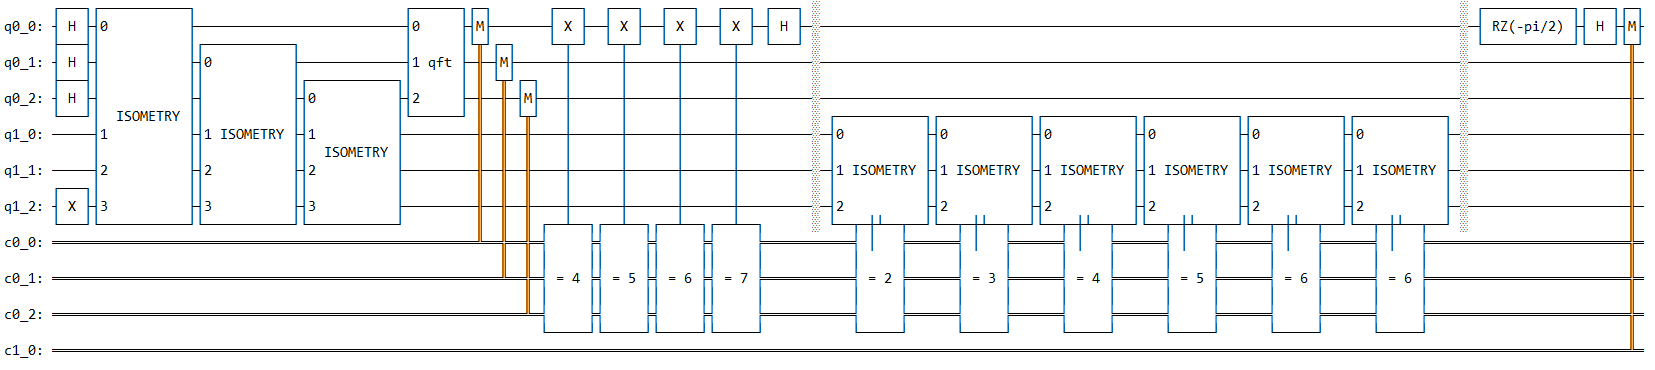
\includegraphics[width=1\linewidth]{oracle}
\caption{Oracle generated from \texttt{oracle(3, 2, 5)}. This circuit estimates $HB_3(2)$ modulo $5$ and puts the value in register \texttt{c1\_0}.}
\end{figure}

\end{frame}

%------------------------------------------------

\begin{frame}{Limitations}

Our oracle works, but is extremely inefficient. Sources of inefficiency:

\begin{itemize}
    \item Unitary matrices used within the oracle are constructed on-the-fly. Their size is exponential in the input size.
    \item Qiskit does not allow the result of a classical measurement to dictate how the rest of the circuit is constructed.
    \item Due to current hardware limitations, this means our oracle can only run in simulators.
\end{itemize}

\begin{figure}
\begin{minipage}[c]{0.67\textwidth}
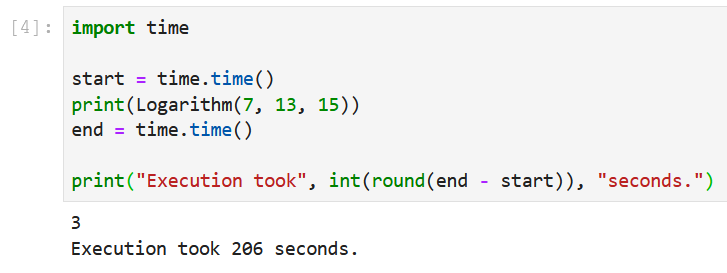
\includegraphics[width=\textwidth]{inefficient}
\end{minipage}\hfill
\begin{minipage}[c]{0.3\textwidth}
\caption{
Our algorithm took 206 seconds to determine that $m=3$ is the value that satisfies $7^m = 13 \mod 15$.
}
\end{minipage}
\end{figure}

\end{frame}

%------------------------------------------------

\begin{frame}{Future Work}

\begin{itemize}
    \item Improve efficiency of the oracle.
    \begin{itemize}
        \item Look into the \texttt{QuantumCircuit.snapshot()} method to improve efficiency on simulators.
        \item Increase efficiency of unitary generation.
    \end{itemize}
    \item Build this into an accessible tutorial explaining the quantum algorithm.
    \item Create a toy demonstration using this algorithm to break RSA encryption.
\end{itemize}
    
\end{frame}

%------------------------------------------------

\begin{frame}{References}
\footnotesize{}
\begin{thebibliography}{99}

\bibitem[Kaliski, 1988]{logarithm} Burton S. Kaliski Jr. (1988)
\newblock Elliptic Curves and Cryptography: A Pseudorandom Bit Generator and Other Tools
\newblock Doctoral dissertation, MIT, Cambridge, USA.
\newblock \href{https://dspace.mit.edu/bitstream/handle/1721.1/14709/18494044-MIT.pdf}{https://dspace.mit.edu/bitstream/handle/1721.1/14709/18494044-MIT.pdf}

\bibitem[Kaliski, 2017]{oracle} Burton S. Kaliski Jr. (2017)
\newblock A Quantum ``Magic Box'' for the Discrete Logarithm Problem
\newblock Cryptology EPrint Archive, Report 2017/745.
\newblock \href{https://eprint.iacr.org/2017/745}{https://eprint.iacr.org/2017/745}

\end{thebibliography}

\end{frame}

%------------------------------------------------

\begin{frame}
\huge{\centerline{The End}}

\begin{center}
{\large A huge thank you to IBM Quantum, the Qiskit community, and the organizers of the North Carolina Qiskit Community Summer Jam 2020 for making this project possible!}
\end{center}

\end{frame}

%-------------------------------------------------

\end{document} 